\documentclass{article} % For LaTeX2e
\usepackage{nips15submit_e,times}
\usepackage{hyperref}
\usepackage{url}
\usepackage{graphicx}
\usepackage{float}
\usepackage{amsmath}
\usepackage{caption}
\usepackage{subcaption}

\usepackage[pdftex]{}
% \documentstyle[nips14submit_09,times,art10]{article} % For LaTeX 2.09


\title{Exploration of Multi-layer Neural Networks on FashionMNIST Classification Tasks}

\author{
Varun Viswanath \\
Department of Electrical and Computer Engineering\\
University of California, San Diego\\
San Diego, CA 92126 \\
\texttt{varunv9@eng.ucsd.edu} \\
\AND
Jorge  Avila \\
Department of Computer Science and Engineering\\
University of California, San Diego\\
San Diego, CA 92126 \\
\texttt{j3avila@eng.ucsd.edu} \\
\AND
Chaoqi Xu \\
Department of Computer Science and Engineering\\
University of California, San Diego\\
San Diego, CA 92126 \\
\texttt{chx001@eng.ucsd.edu} \\
}

% The \author macro works with any number of authors. There are two commands
% used to separate the names and addresses of multiple authors: \And and \AND.
%
% Using \And between authors leaves it to \LaTeX{} to determine where to break
% the lines. Using \AND forces a linebreak at that point. So, if \LaTeX{}
% puts 3 of 4 authors names on the first line, and the last on the second
% line, try using \AND instead of \And before the third author name.

\newcommand{\fix}{\marginpar{FIX}}
\newcommand{\new}{\marginpar{NEW}}

\nipsfinalcopy % Uncomment for camera-ready version

\begin{document}

\maketitle

\begin{abstract}
Fashion object classification is a representative field of much of object recognition. Fashion objects are diverse in shape, color, and material similar to how real-world objects in general vary in shape, color and material. Strong performance and error analysis on this dataset could result in important improvements for object recognition and computer vision as a whole. We explored the use of a multi-layer neural network trained on raw pixel values of the FashionMNIST dataset. We explore various hyper-parameter settings and network configurations for approaching this task, achieving a final testing accuracy of BLANK with a BLANK neural network. As our model overfit to the training data, we suggest increasing variability in the dataset. We conclude that BLANK is the best configuration of a multi-layer neural network classifier for the FashionMNIST dataset.
\end{abstract}


\section{Classification Experiments}

\subsection{Data loading (3.a)}
We implement data loading and normalization with $$\text{normalized data} = \frac{\text{data} - \text{mean}(\text{data})}{\text{standard dev}(\text{data})}$$


\subsection{Implmentation and gradient checking} 
Next, we implement the classification algorithm and perform the gradient check to confirm our forwards and backwards pass implementations. We use epsilon=1e-1 so we check that the differences are less than 1e-2. See \ref{table:table 1.}

\begin{table}[h!]
\centering
\begin{tabular}{|c c c | c c | c |} 
 \hline
Layer & Type & Index & Approx & Actual & Diff\\ [0.5ex] 
 \hline\hline
 0 & bias & 15 & -0.082962 & -0.082686 & 0.000276 \\ 
 2 & bias & 0 & 0.142779 & 0.142924 & 0.000145\\
 0 & weight & 2, 15 & 0.067220 & 0.067073  & 0.000147\\
 0 & weight & 9, 12 & -0.061648 & -0.061630 & 0.000018 \\
 2 & weight & 4, 7 & 0.096074 & 0.096129 & 0.000055\\ 
 2 & weight & 7, 4 & -0.120126 & -0.120196 & 0.000071\\ 
 \hline
\end{tabular}
\caption{Table to show that variation between gradients and their approximation are less than the variations squared. Here each weight was varied by 1e-1, and all differences are less than 1e-2 or 0.01 }
\label{table:1}
\end{table}

As you can see, all differences are much less than 0.01. So, all weights pass the gradient check.

\subsection{Tuning Learning rate (3.c)} 
We implemented mini-batch stochastic gradient descent, momentum, cross-validation, and early stopping.

Our training procedure is as follows. We begin by loading the data, and normalizing, centering, and standardizing the inputs using the formula describe above. Next we split the training data in validation and training datasets, keeping 20\% of the data for cross-validation and early stopping. We then begin training the model for 100 epochs, stopping early if the validation loss increases for 5 epochs in a row and recording the training and validation loss and accuracy, as well as a copy of the model itself. In each epoch, we first randomly shuffle the training data, and then iterate through mini-batches, each with 128 examples, performing a model forward pass and backwards pass for each mini-batch. Forward passes are described by $$z_{layer+1} = g(w^T z_{layer} + b)$$ for each layer. For each backwards pass, we first calculated the gradient with respect to the cross entropy loss and softmax function, which is
$$\delta_k = t - y$$ and then we back propagate this gradient through each layer. Weights and biases are updated with momentum, $\mu$, as  \\
$$w_{layer} = w_{layer} - \alpha( \delta_{layer} z_{layer} + \mu (\text{previous-gradient}))$$
$$b_{layer} = b_{layer} - \alpha (\delta_{layer} z_{layer} + \mu (\text{previous-gradient}))$$
and delta's are back propagated as 
$$\delta_{layer -1} = \delta_{layer} w_{layer}$$

After completing our implementation, we went on to pick the best learning rate from our experiments. Below we present our best loss and accuracy

% ====== Loss and Accuracy figure Start ======
\begin{figure}[H]
\centering
\begin{subfigure}{.5\textwidth}
  \centering
  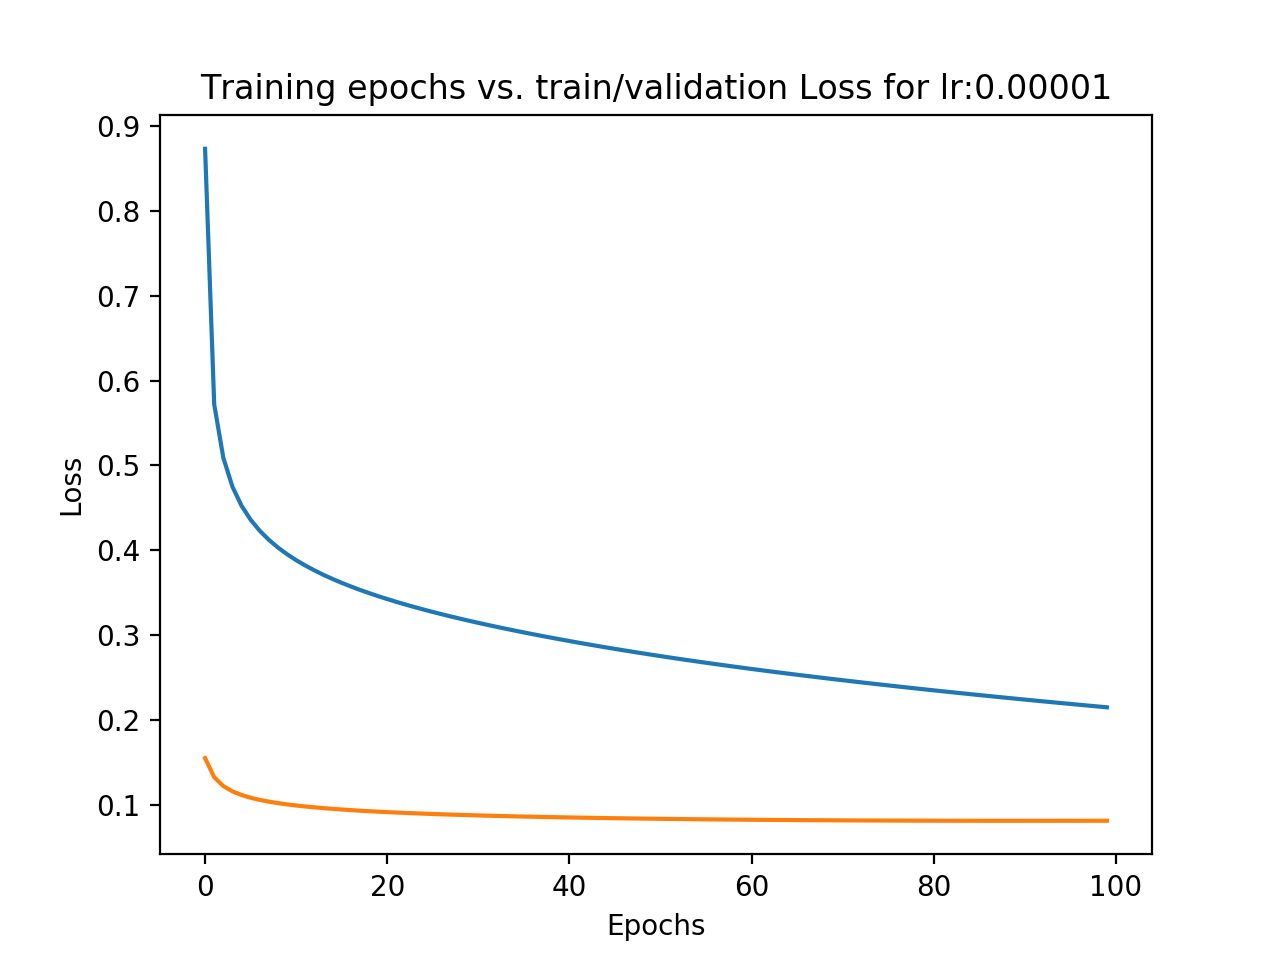
\includegraphics[width=0.95\linewidth]{3c/3c_lr00001_loss.png}
  \label{fig:sub1}
\end{subfigure}%
\begin{subfigure}{.5\textwidth}
  \centering
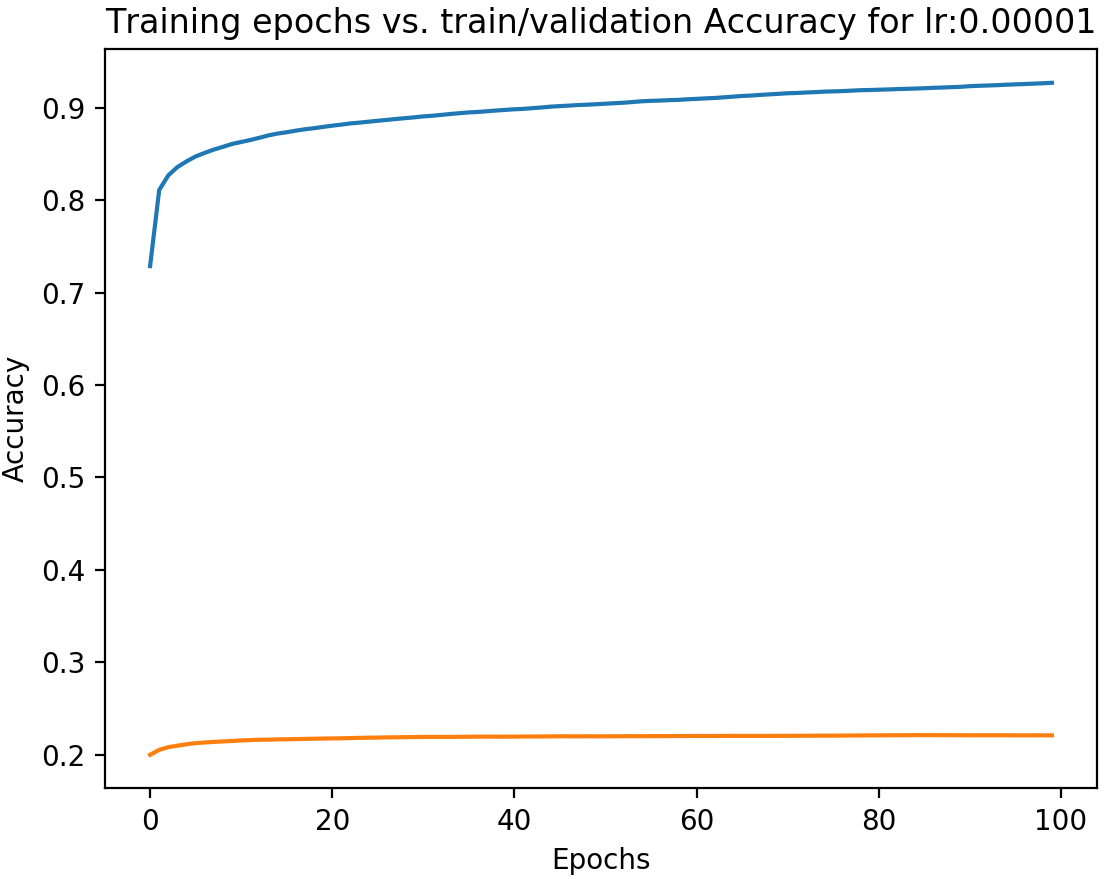
\includegraphics[width=0.95\linewidth]{3c/3c_lr00001_acc.png}
  \label{fig:sub2}
\end{subfigure}
\caption{Training(blue) and Validation(Orange) Loss and Accuracy of Multi-Layer Neural Network classifier with learning rate 0.00001}
\label{fig:test}
\end{figure}
% ====== Loss and Accuracy figure End ======

With this learning rate we achieved a testing set loss of 0.072554 and accuracy of 0.182580.

\subsection{Implement and tune weight decay (3.d)}
Next, we implement weight decay for the above model. We experiment with weight decay penalties of 0.001 and 0.0001. We present our findings below.

% ====== Loss and Accuracy figure Start (0.001)======
\begin{figure}[H]
\centering
\begin{subfigure}{.5\textwidth}
  \centering
  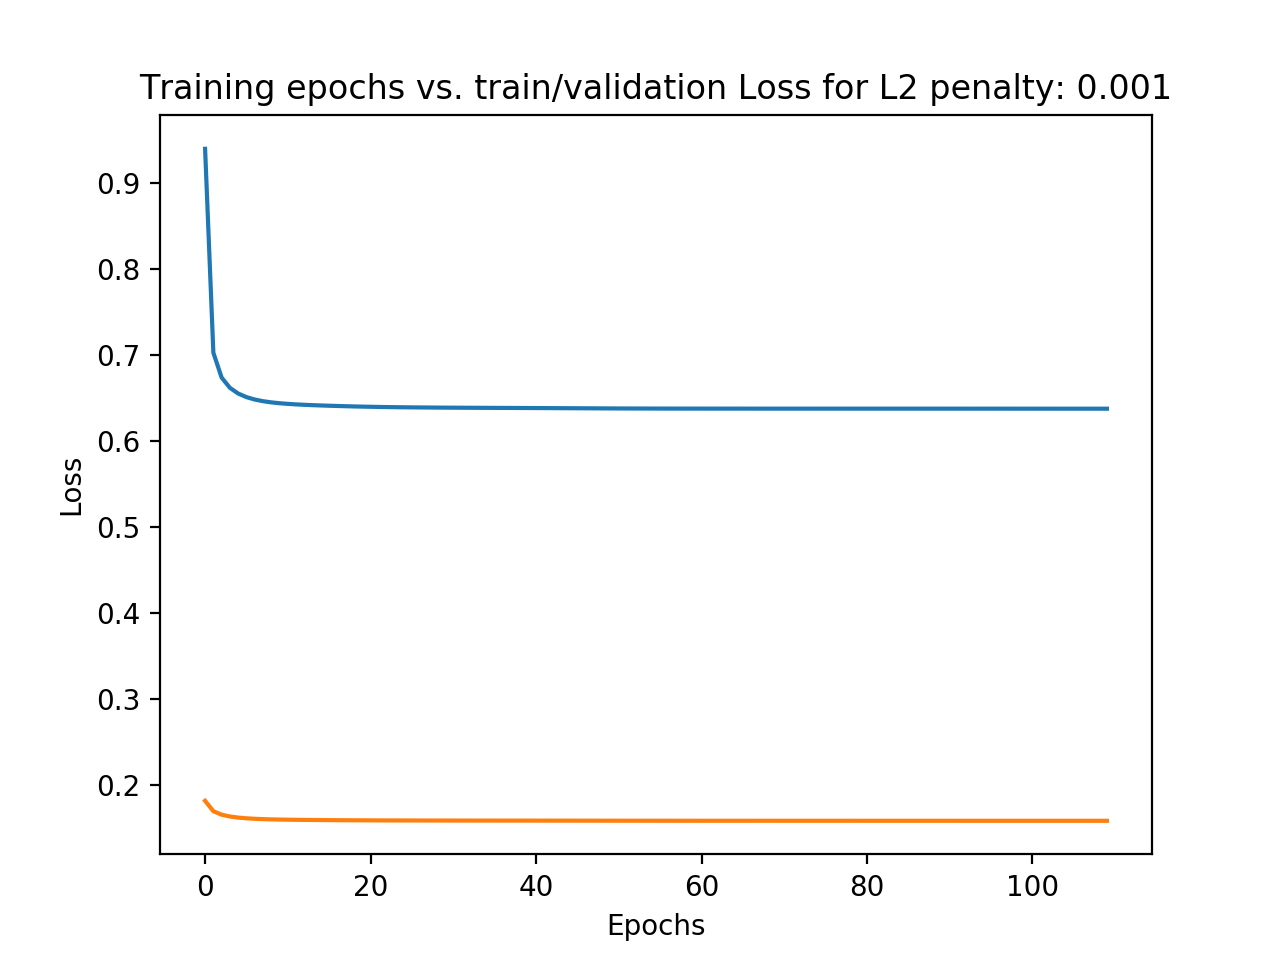
\includegraphics[width=0.95\linewidth]{3d/3d_l2p001_loss.png}
  \label{fig:sub1}
\end{subfigure}%
\begin{subfigure}{.5\textwidth}
  \centering
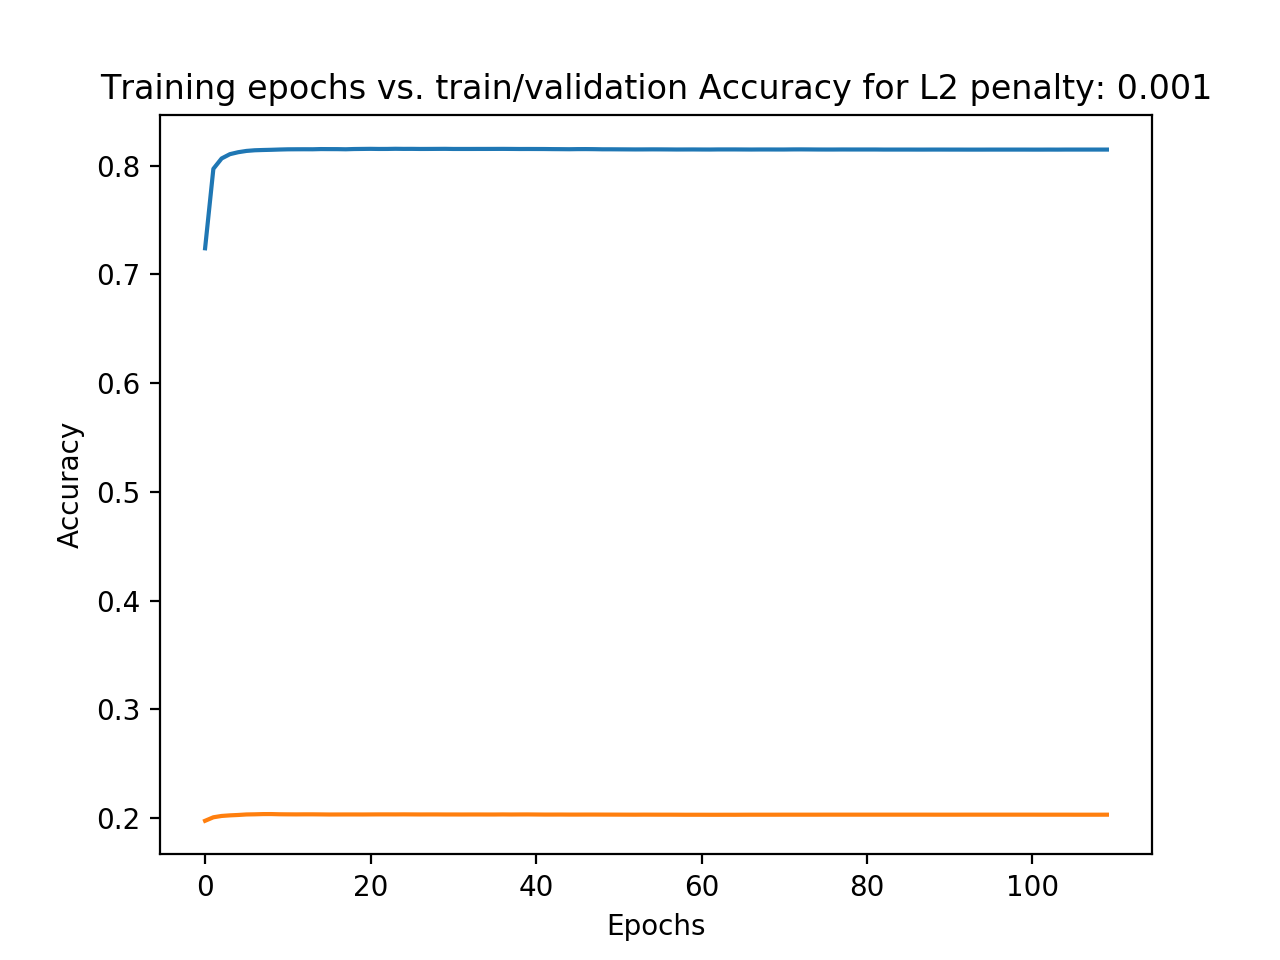
\includegraphics[width=0.95\linewidth]{3d/3d_l2p001_acc.png}
  \label{fig:sub2}
\end{subfigure}
\caption{Training(blue) and Validation(Orange) Loss and Accuracy of Multi-Layer Neural Network classifier with an L2 Regularization penalty of 0.001}
\label{fig:test}
\end{figure}
% ====== Loss and Accuracy figure End ======

% ====== Loss and Accuracy figure Start (0.0001) ======
\begin{figure}[H]
\centering
\begin{subfigure}{.5\textwidth}
  \centering
  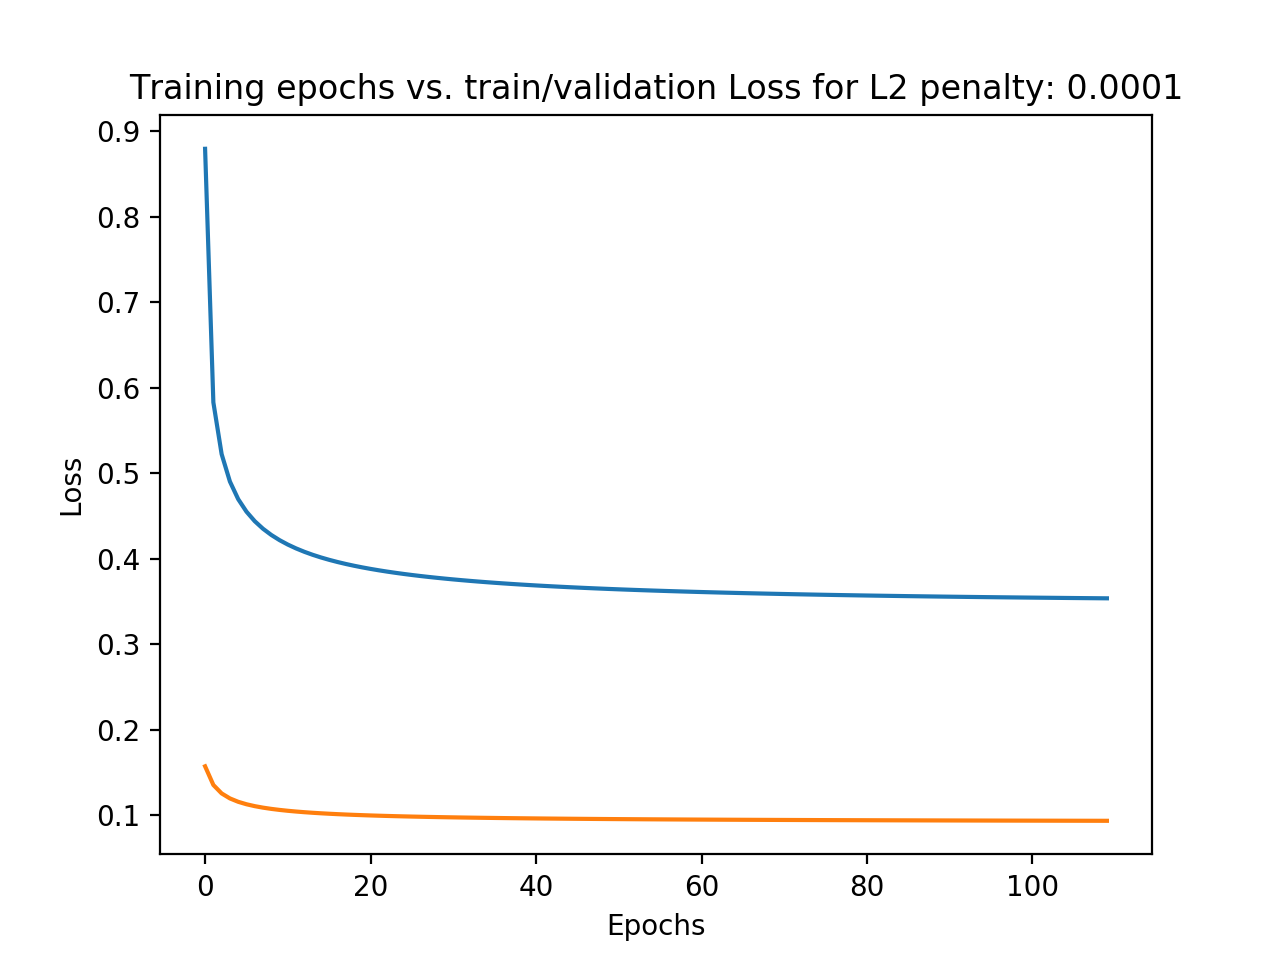
\includegraphics[width=0.95\linewidth]{3d/3d_l2p0001_loss.png}
  \label{fig:sub1}
\end{subfigure}%
\begin{subfigure}{.5\textwidth}
  \centering
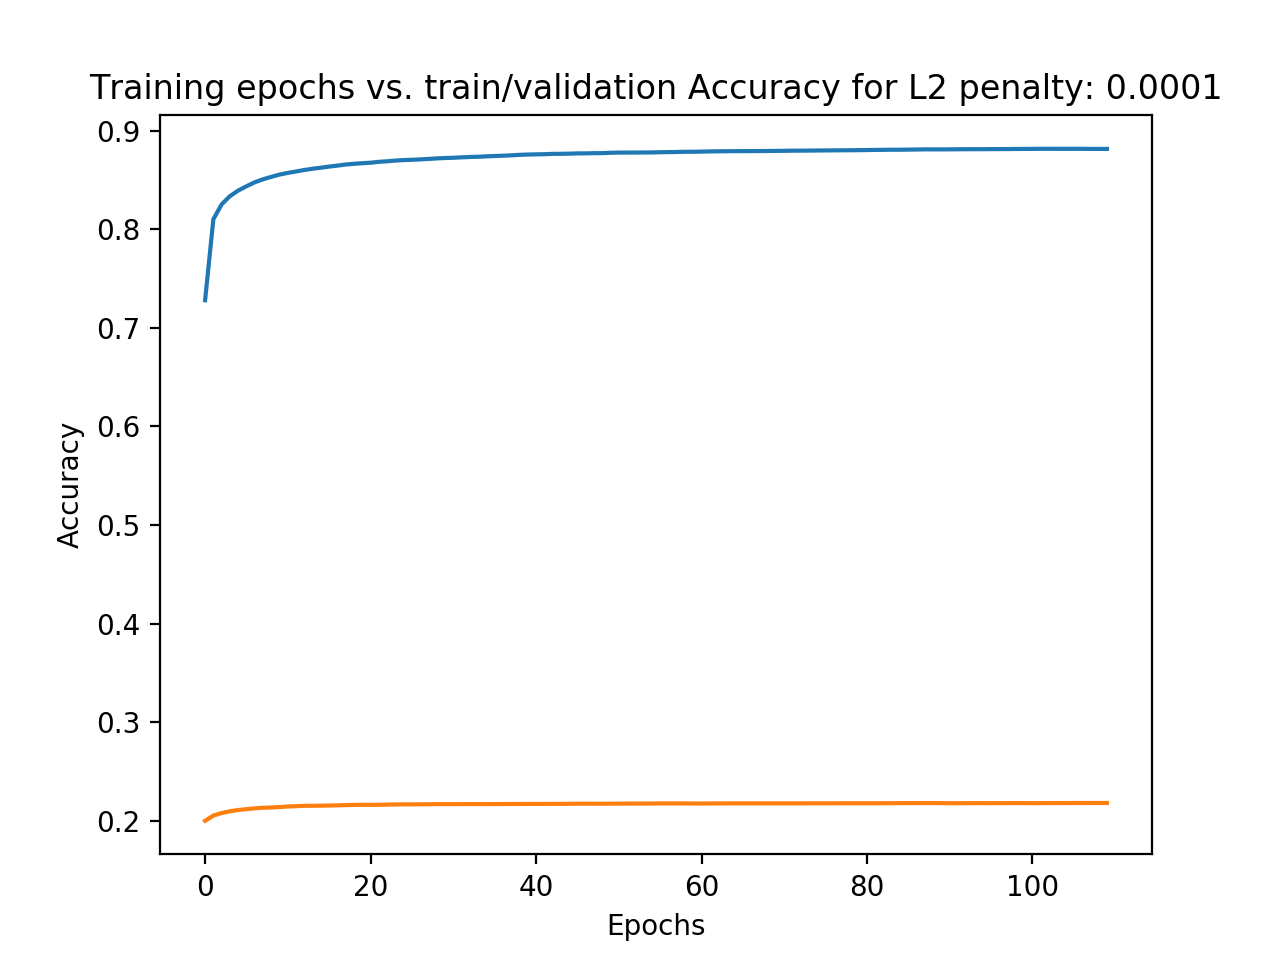
\includegraphics[width=0.95\linewidth]{3d/3d_l2p0001_acc.png}
  \label{fig:sub2}
\end{subfigure}
\caption{Training(blue) and Validation(Orange) Loss and Accuracy of Multi-Layer Neural Network classifier with an L2 Regularization penalty of 0.0001}
\label{fig:test}
\end{figure}
% ====== Loss and Accuracy figure End ======

The best performing parameter setting was 0.0001 with a final testing set loss of 0.083761 and accuracy of 0.179059

\subsection{ (3.e)}
Next, we implement various activation functions for the above model. We experiment with the sigmoid activation function and the ReLU activation function. We calculate gradients for the sigmoid functions using $$\Delta \text{sigmoid} = \text{sigmoid}(z)*(1-\text{sigmoid}(z))$$ and for the ReLU function using $$\Delta \text{ReLU} = \begin{cases} 
      0 & x\leq 0 \\
      1 & x > 0 
  \end{cases}
$$ We present our findings below. 

% ====== Loss and Accuracy figure Start sigmoid) ======
\begin{figure}[H]
\centering
\begin{subfigure}{.5\textwidth}
  \centering
  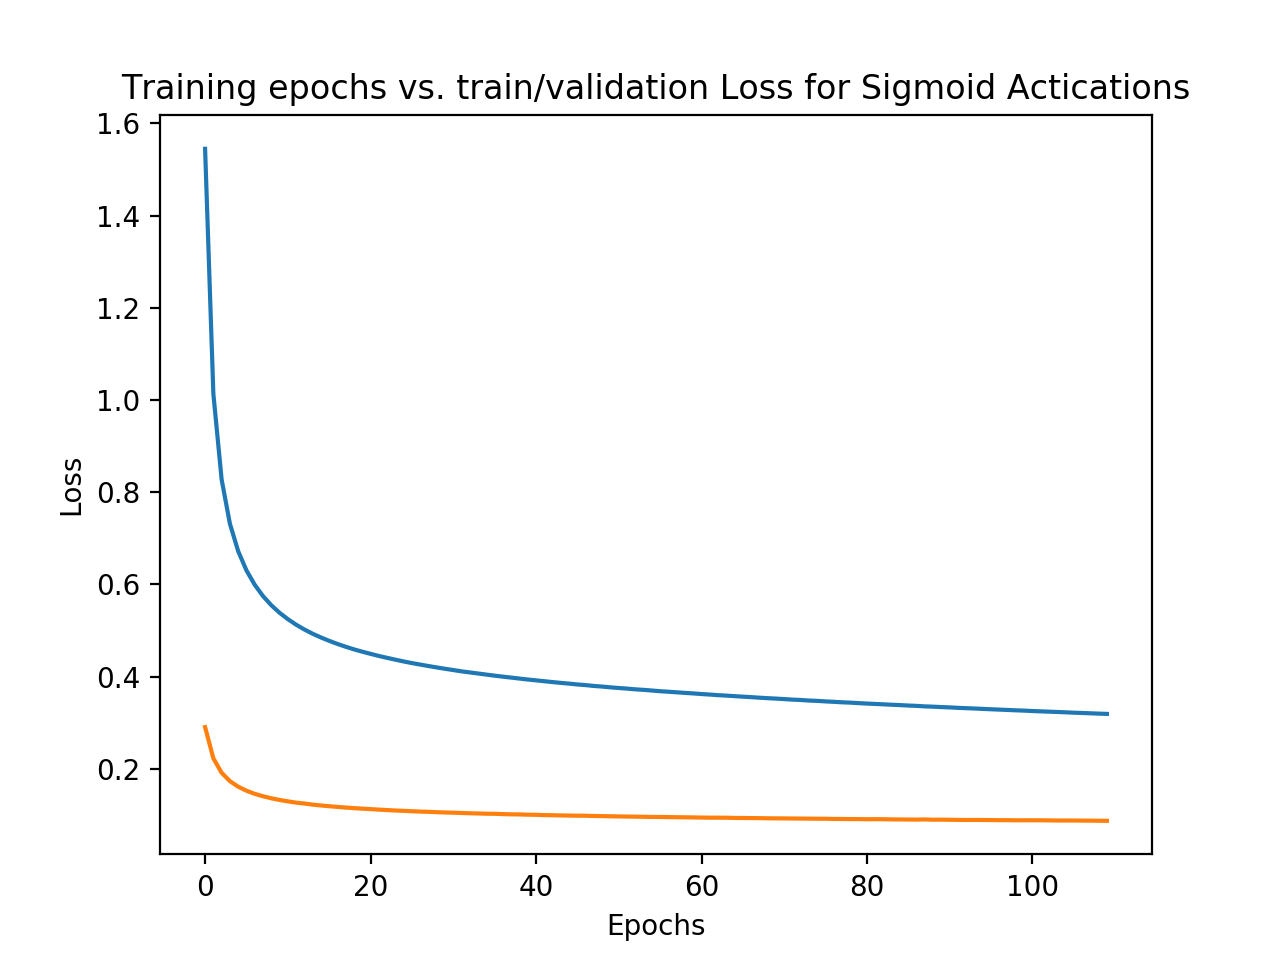
\includegraphics[width=0.95\linewidth]{3e/3e_sig_loss.png}
  \label{fig:sub1}
\end{subfigure}%
\begin{subfigure}{.5\textwidth}
  \centering
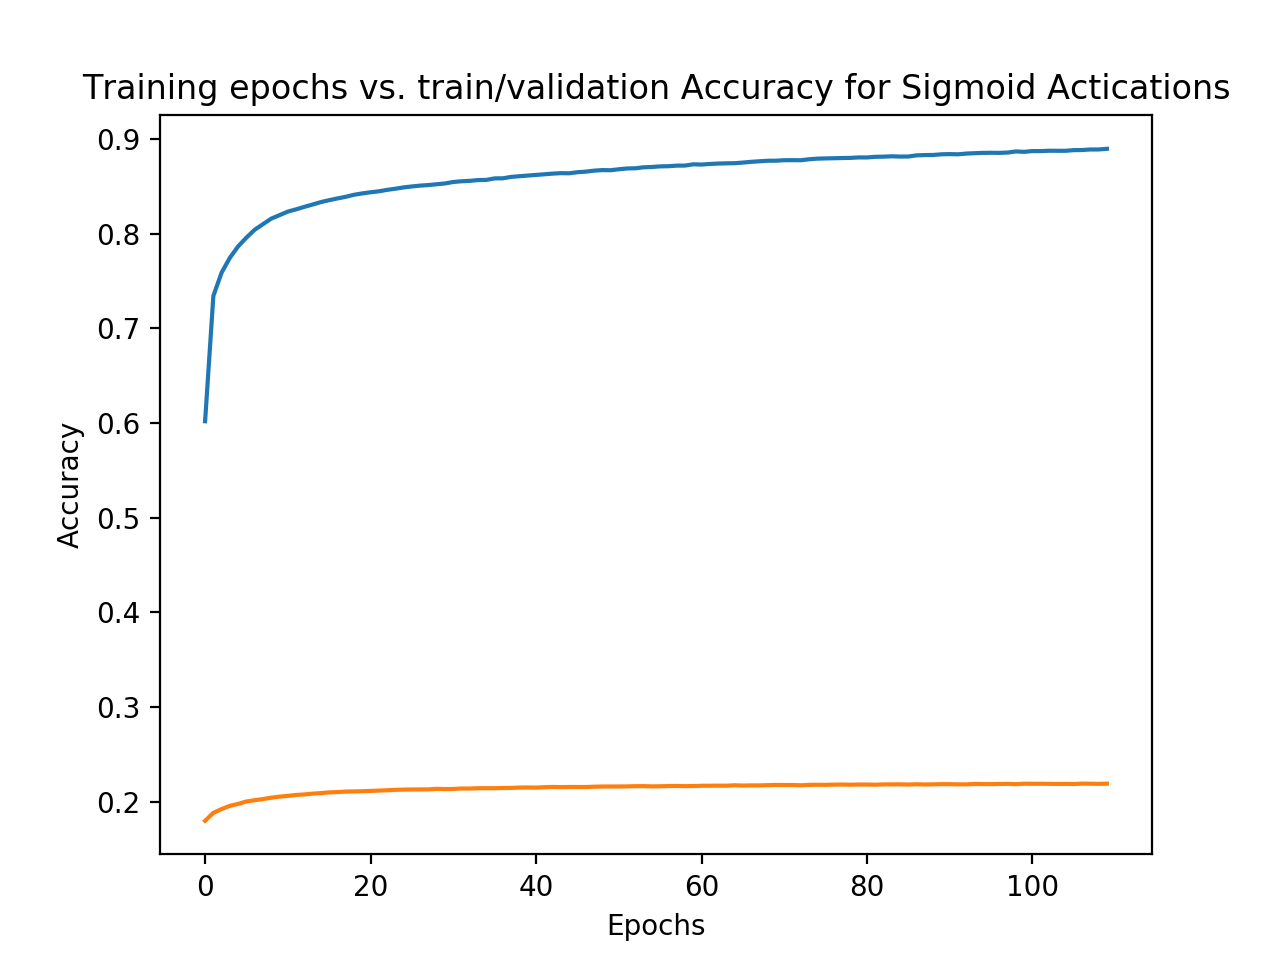
\includegraphics[width=0.95\linewidth]{3e/3e_sig_acc.png}
  \label{fig:sub2}
\end{subfigure}
\caption{Training(blue) and Validation(Orange) Loss and Accuracy of Multi-Layer Neural Network classifier with Sigmoid activation functions between layers}
\label{fig:test}
\end{figure}
% ====== Loss and Accuracy figure End ======

% ====== Loss and Accuracy figure Start relu) ======
\begin{figure}[H]
\centering
\begin{subfigure}{.5\textwidth}
  \centering
  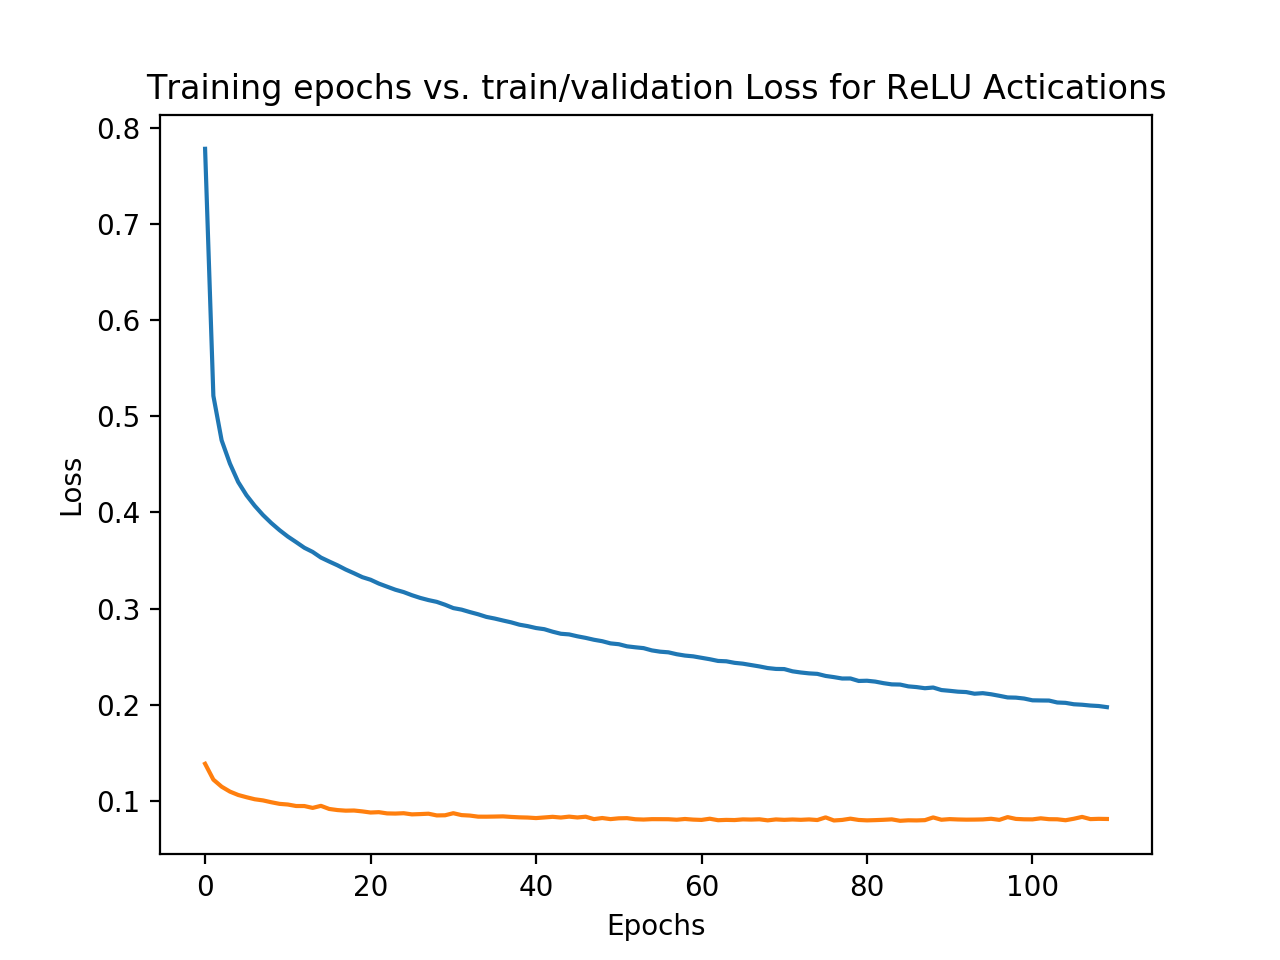
\includegraphics[width=0.95\linewidth]{3e/3e_relu_loss.png}  \label{fig:sub1}
\end{subfigure}%
\begin{subfigure}{.5\textwidth}
  \centering
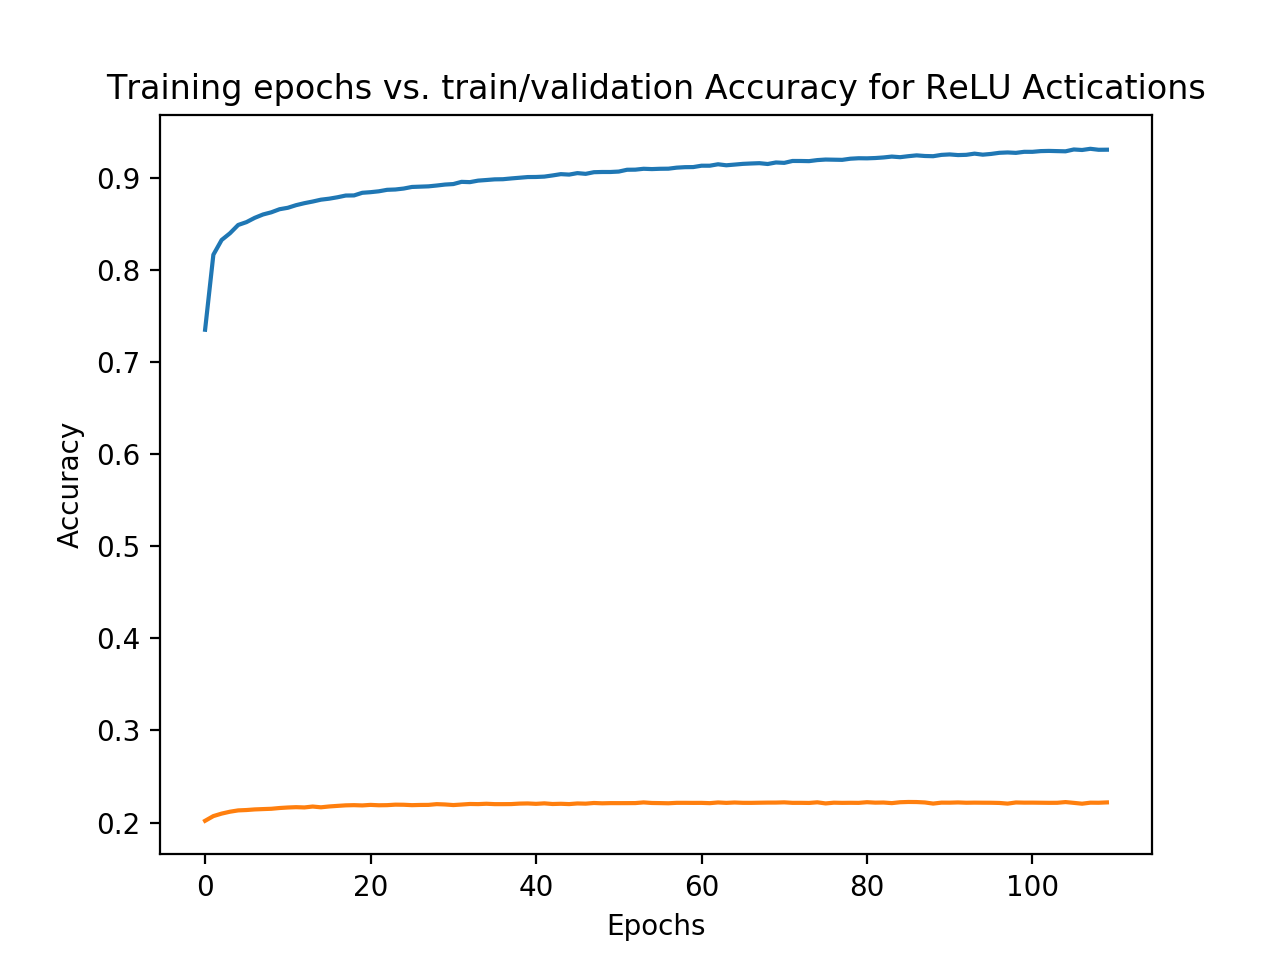
\includegraphics[width=0.95\linewidth]{3e/3e_relu_acc.png}
  \label{fig:sub2}
\end{subfigure}
\caption{Training(blue) and Validation(Orange) Loss and Accuracy of Multi-Layer Neural Network classifier with a ReLU activation functions between layers}
\label{fig:test}
\end{figure}
% ====== Loss and Accuracy figure End ======

The best performing activation function was the ReLU activation with a final testing set loss of 0.076100 and accuracy of 0.182892

\subsection{Network Topology experiments (3.f)}

Finally, we implement various network topologies for the above model. We experiment with 25 hidden units, 100 hidden units, and 2 hidden layers each with 25 hidden units. We present our findings below. 

% ====== Loss and Accuracy figure Start (25 h) ======
\begin{figure}[H]
\centering
\begin{subfigure}{.5\textwidth}
  \centering
  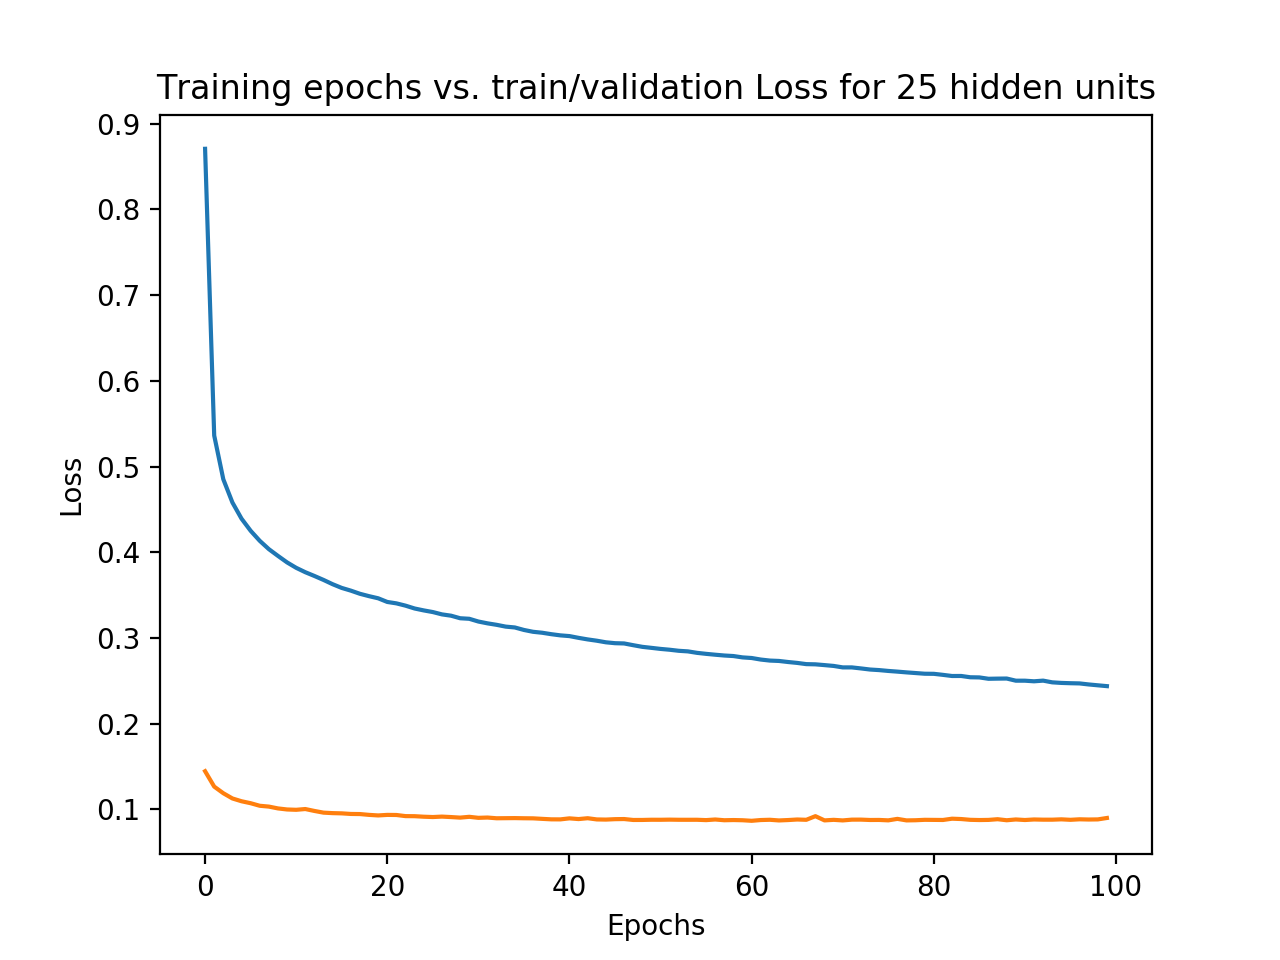
\includegraphics[width=0.95\linewidth]{3f/3f_h25_loss.png}  \label{fig:sub1}
\end{subfigure}%
\begin{subfigure}{.5\textwidth}
  \centering
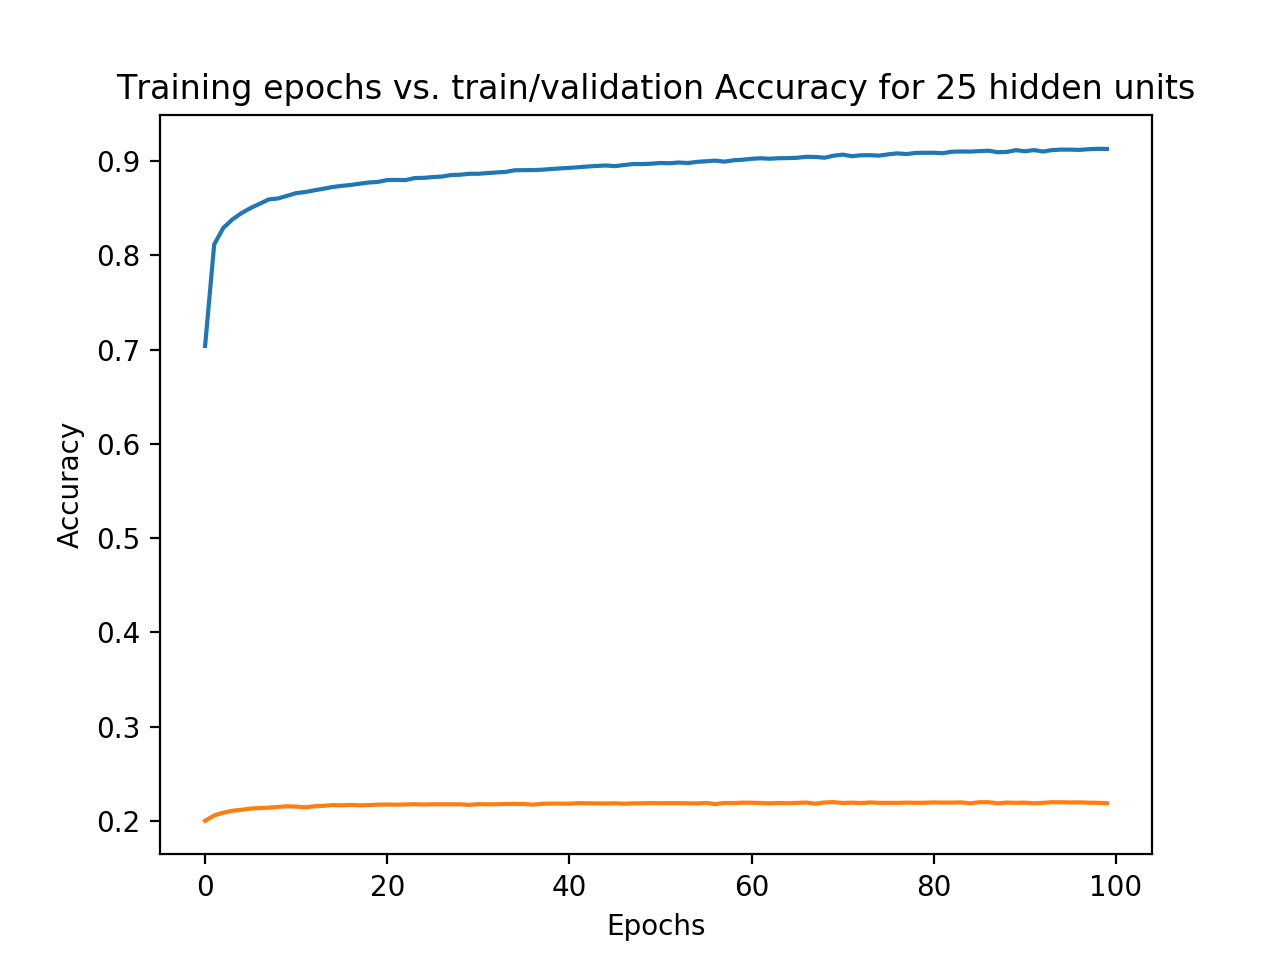
\includegraphics[width=0.95\linewidth]{3f/3f_h25_acc.png}
  \label{fig:sub2}
\end{subfigure}
\caption{Training(blue) and Validation(Orange) Loss and Accuracy of Multi-Layer Neural Network classifier with a 25 unit hidden layer}
\label{fig:test}
\end{figure}
% ====== Loss and Accuracy figure End ======

% ====== Loss and Accuracy figure Start (100 h) ======
\begin{figure}[H]
\centering
\begin{subfigure}{.5\textwidth}
  \centering
  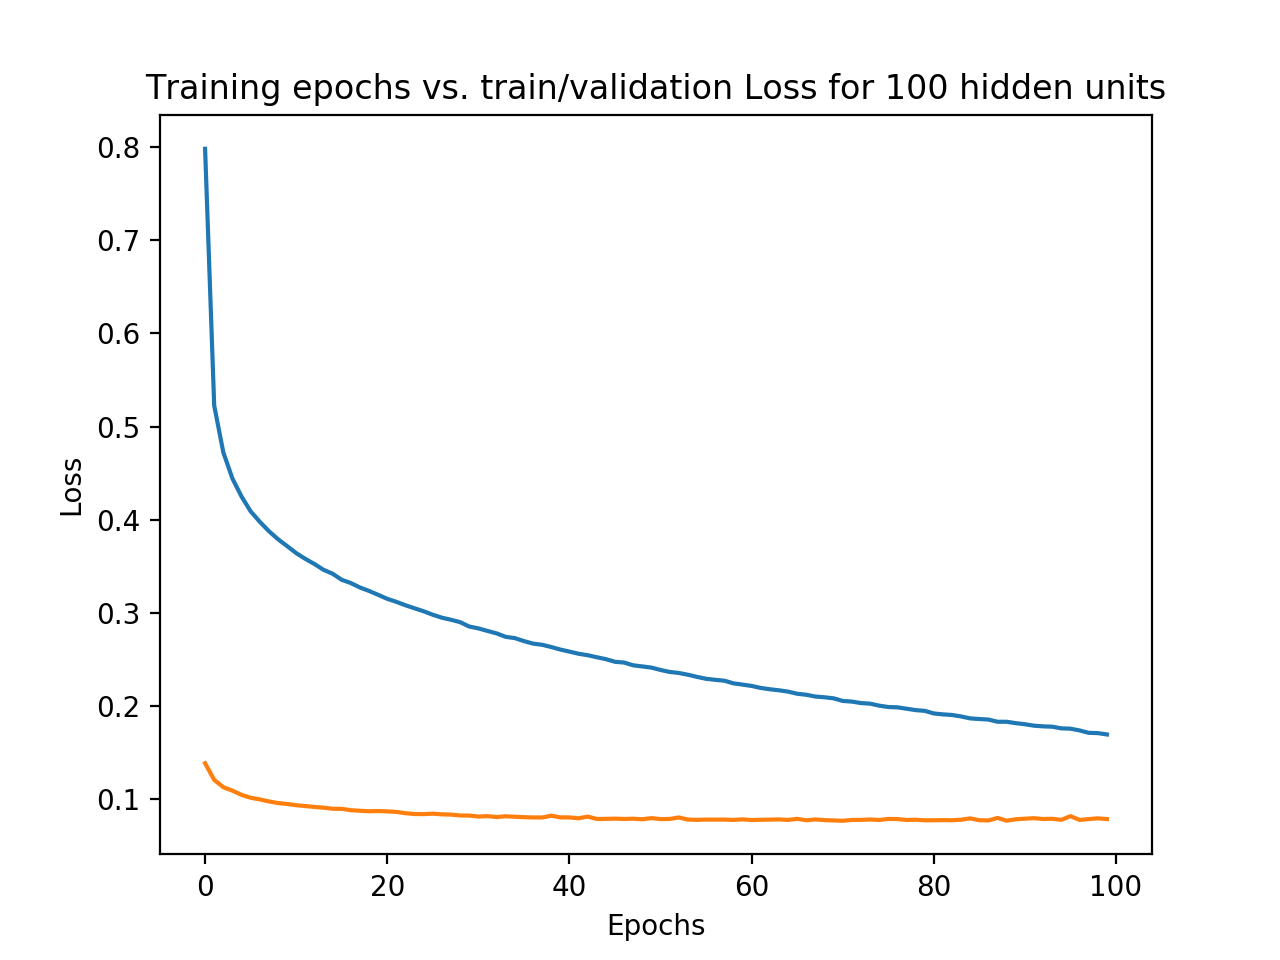
\includegraphics[width=0.95\linewidth]{3f/3f_h100_loss.png}  \label{fig:sub1}
\end{subfigure}%
\begin{subfigure}{.5\textwidth}
  \centering
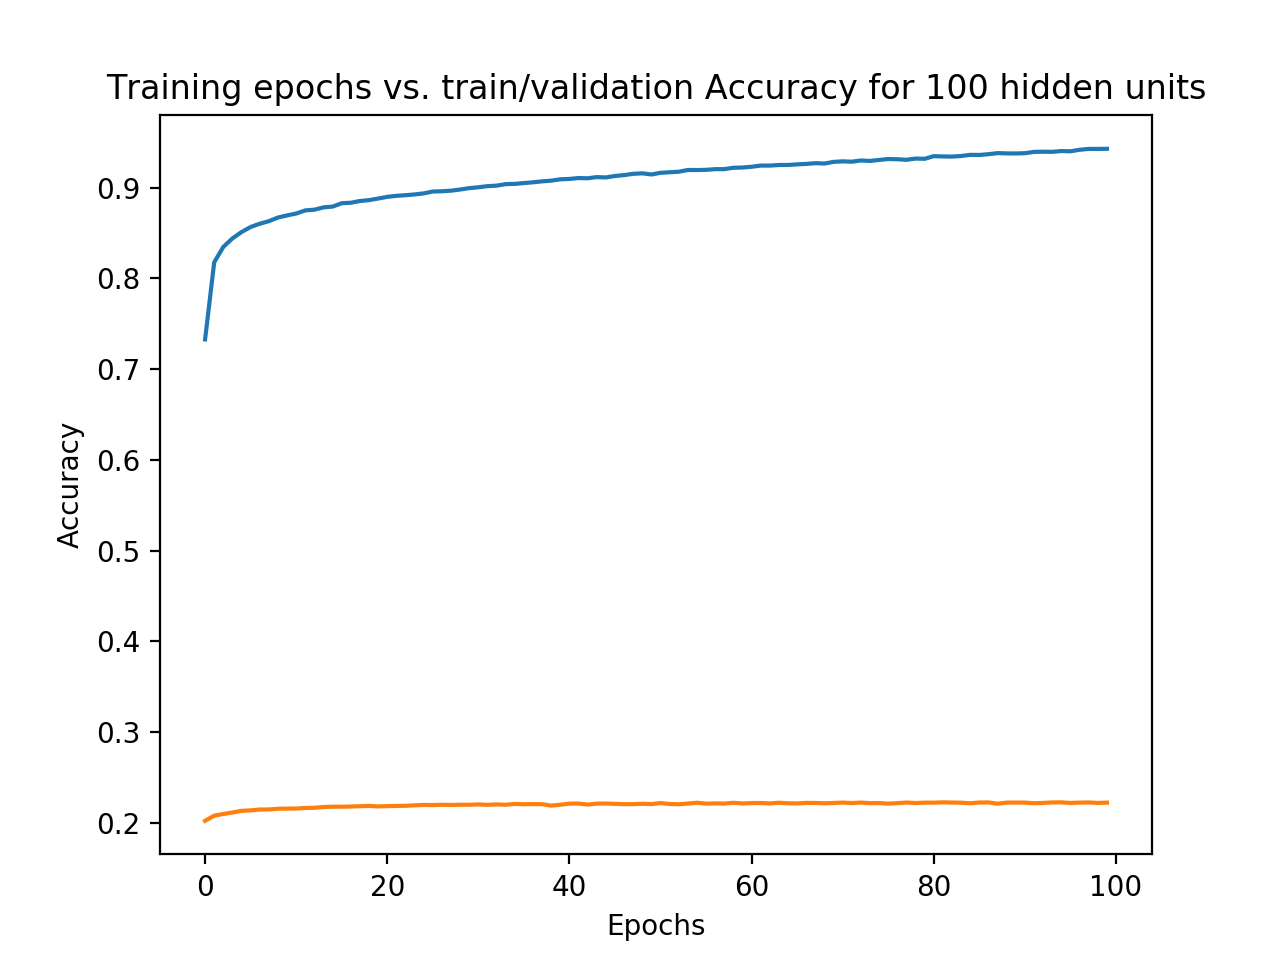
\includegraphics[width=0.95\linewidth]{3f/3f_h100_acc.png}
  \label{fig:sub2}
\end{subfigure}
\caption{Training(blue) and Validation(Orange) Loss and Accuracy of Multi-Layer Neural Network classifier with a 100 unit hidden layer}
\label{fig:test}
\end{figure}
% ====== Loss and Accuracy figure End ======

% ====== Loss and Accuracy figure Start (2 25 h) ======
\begin{figure}[H]
\centering
\begin{subfigure}{.5\textwidth}
  \centering
  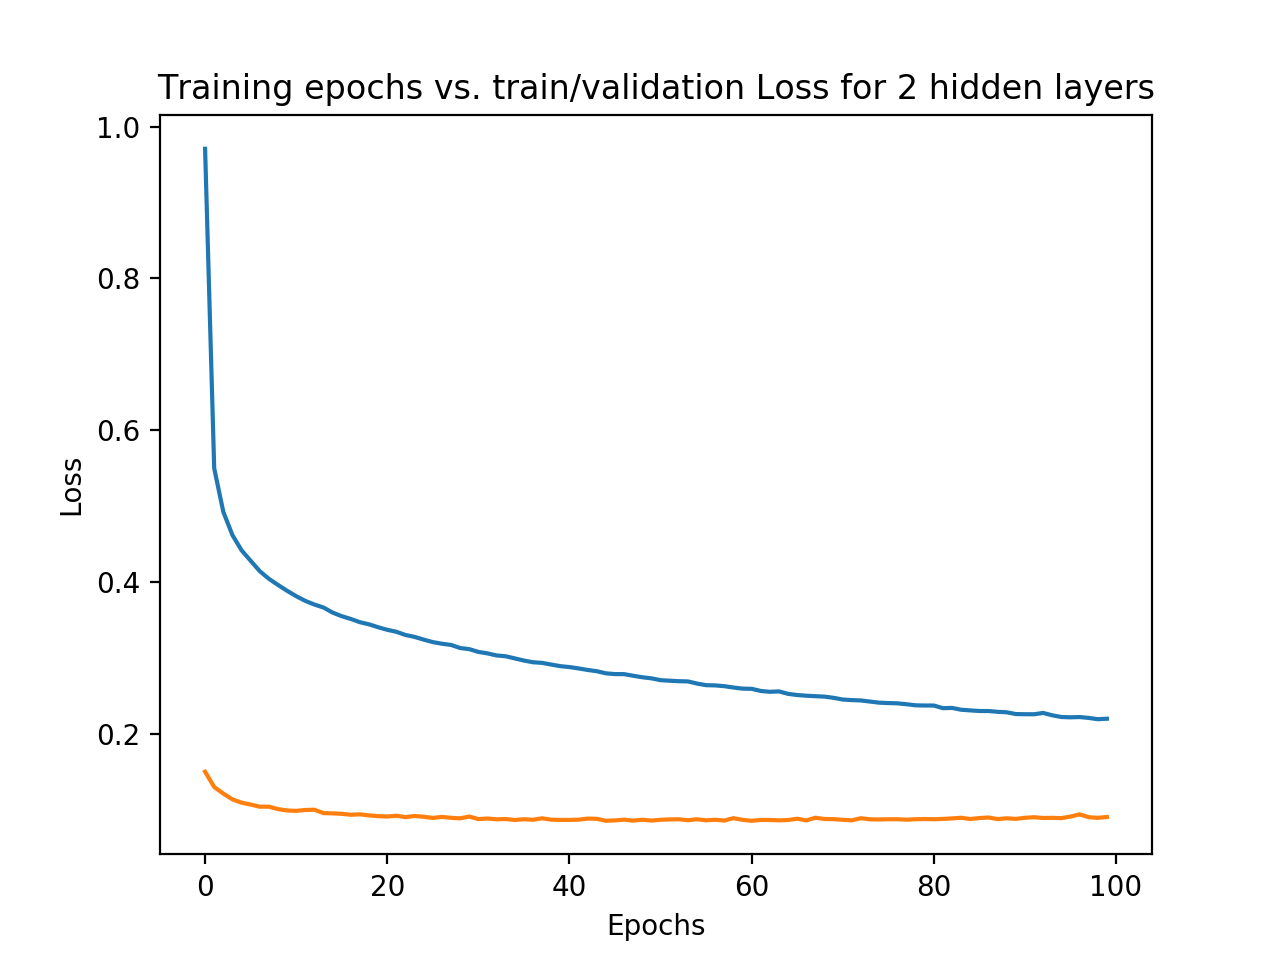
\includegraphics[width=0.95\linewidth]{3f/3f_2h25_loss.png}  \label{fig:sub1}
\end{subfigure}%
\begin{subfigure}{.5\textwidth}
  \centering
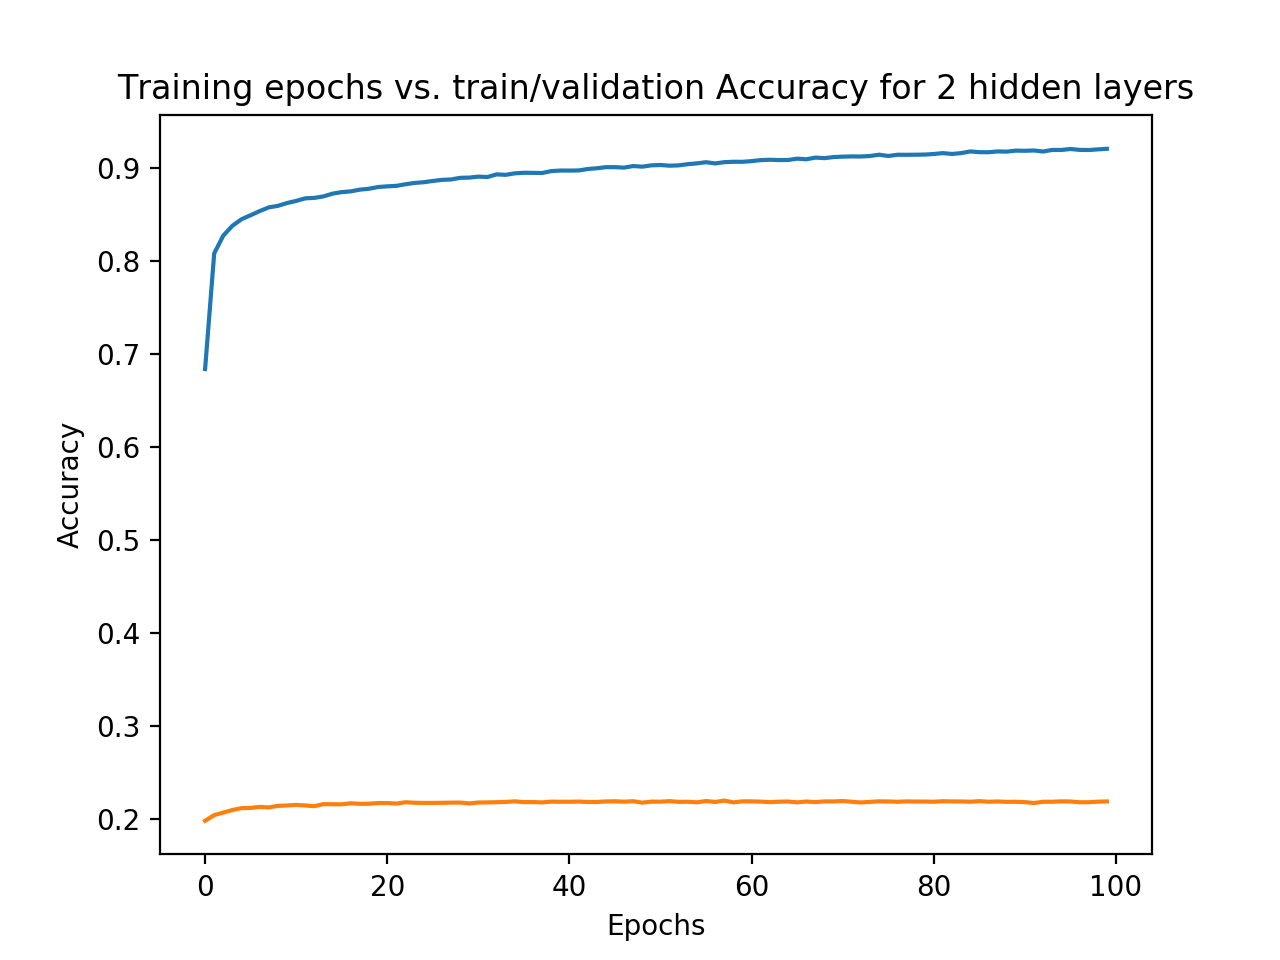
\includegraphics[width=0.95\linewidth]{3f/3f_2h25_acc.png}
  \label{fig:sub2}
\end{subfigure}
\caption{Training(blue) and Validation(Orange) Loss and Accuracy of Multi-Layer Neural Network classifier with 2 25 unit hidden layers}
\label{fig:test}
\end{figure}
% ====== Loss and Accuracy figure End ======

The best performing network architecture was the 100 unit hidden layer with a final test accuracy of 0.184142.

\section{Individual Contributions}
We all worked together on most of the project.

\subsection{Jorge}
My contributions were writing the PCA function, the k-fold cross validation class, and the plotting code. I also helped the whole team with debugging, cleaning, and structuring code.

\subsection{Varun}
My contributions were writing the logistic regression function. I also helped the whole team with debugging, cleaning, and structuring code.

\subsection{Chaoqi}
My contributions were writing the Softmax regression function. I also helped the whole team with debugging, cleaning, and structuring code.


\end{document}
